\documentclass{standalone}
\usepackage{tikz}
\usetikzlibrary{decorations.pathmorphing, arrows.meta}

\begin{document}

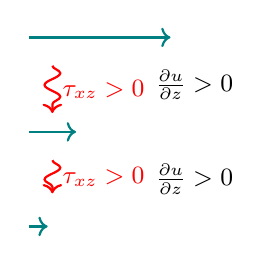
\begin{tikzpicture}[scale=1.2]

    % draw three horizontal arrows for the velocity, with the velocity
    % higher as we go up (du/dz>0).  Make these blue
    \draw[->, teal, thick] (0,2) -- (1.5,2) node[midway, below] {};
    % label du/dz between the arrows:
    \node at (1.75,1.5) {\small $\frac{\partial u}{\partial z} > 0$};
    \draw[->, teal, thick] (0,1) -- (0.5,1) node[midway, below] {};
    \node at (1.75,0.5) {\small $\frac{\partial u}{\partial z} > 0$};
    \draw[->, teal, thick] (0,0) -- (0.2,0) node[midway, below] {};

    % draw squiggly vertical arrow for the shear stress
    \draw[->, decorate, decoration={snake, amplitude=1mm, segment length=3mm}, thick, red]
      (0.25,1.7) -- (0.25,1.2) node[midway, right] {\small $\tau_{xz} > 0$};
    \draw[->, decorate, decoration={snake, amplitude=1mm, segment length=3mm}, thick, red]
      (0.25,0.7) -- (0.25,0.35) node[midway, right] {\small $\tau_{xz} > 0$};


\end{tikzpicture}

\end{document}
